\documentclass[UTF8,fontset=windows,zihao=-4,a4paper]{ctexart}
\usepackage[top=20mm,bottom=20mm,left=22mm,right=22mm]{geometry}
\usepackage{graphicx,xcolor,array,longtable,booktabs,enumitem,fancyhdr,hyperref,fvextra,needspace,xurl}
\definecolor{Green}{HTML}{173D35}
\definecolor{Muted}{HTML}{61766D}
\definecolor{Rule}{HTML}{D8E3DC}
\setmainfont{TeX Gyre Termes}
\setmonofont{Consolas}
\hypersetup{colorlinks=true,linkcolor=Green,urlcolor=Green,bookmarksnumbered=true,pdfauthor={校园活动工作台小组},pdftitle={校园活动工作台 - 用户手册}}
\urlstyle{tt}
\Urlmuskip=0mu plus 1mu
\setlength{\parindent}{0pt}
\setlength{\parskip}{4.5pt}
\linespread{1.15}
\setlist[enumerate]{leftmargin=1.8em,itemsep=3pt,topsep=4pt,parsep=0pt}
\setlength{\LTpre}{5pt}\setlength{\LTpost}{7pt}
\ctexset{section={format=\Large\bfseries\color{Green},beforeskip=16pt,afterskip=7pt},subsection={format=\normalsize\bfseries\color{Green},beforeskip=10pt,afterskip=4pt}}
\pagestyle{fancy}\fancyhf{}
\fancyhead[L]{\small\color{Muted}校园活动工作台}
\fancyhead[R]{\small\color{Muted}用户手册}
\fancyfoot[L]{\footnotesize\color{Muted}v1.0 正式版 · 2026.10.12}
\fancyfoot[R]{\small\color{Green}\thepage}
\setlength{\headheight}{16pt}
\renewcommand{\headrulewidth}{0.3pt}
\renewcommand{\footrulewidth}{0pt}
\raggedbottom
\begin{document}
{\small\color{Muted}校园活动工作台 / 使用与操作}\par\vspace{4pt}
{\huge\bfseries\color{Green}用户手册}\par\vspace{5pt}
{\color{Green}\rule{\linewidth}{1.2pt}}\par
适用版本：v1.0 正式版，功能基线 d39138e。更新日期：2026 年 10 月 12 日。


本手册面向活动组织者、协作成员和服务人员，按“建项目 → 做计划 → 安排人员与资源 → 执行验收 → 收尾归档”的顺序介绍操作。安装、联网和备份恢复见同目录《运维指南》。截图采用校园科技文化节示例，操作时填写自己的活动信息。


\Needspace{10\baselineskip}\section{首次使用：启动、登录与建项目}\label{sec:1}

\Needspace{4\baselineskip}\subsection*{启动与停止}

安装 Node.js 18 或更高版本后，在仓库根目录双击 \path{start.bat}，浏览器会打开 {\def\UrlBreaks{\do\/}\path{http://127.0.0.1:4175/}}。保持启动窗口运行；结束时在窗口按 Ctrl+C，或双击 \path{stop.bat}。也可以在仓库根目录执行：


\Needspace{4\baselineskip}

\begin{Verbatim}[fontsize=\small,breaklines=true,breakanywhere=true,frame=single,rulecolor=\color{Rule},framesep=7pt]

node workbench/demo2/server.mjs

\end{Verbatim}

无需安装额外运行依赖。完整功能从上述服务地址进入。


\Needspace{4\baselineskip}\subsection*{登录与身份}

\begin{enumerate}[start=1]

\item 首次使用选择注册。账号为 3 至 60 位字母、数字或 \path{_.-}，密码为 8 至 128 位。

\item 组织者选择“组织活动”；服务人员选择“参加服务”。填写姓名、联系方式、学院或部门、技能、可服务时段。

\item 组织者登录后进入项目库；服务人员进入个人任务页，也可访问 {\def\UrlBreaks{\do\/}\path{http://127.0.0.1:4175/staff.html}}。

\item 在个人资料入口修改信息。重新打开项目时，资料更新到名册，原资格、排班与考勤记录保留。

\end{enumerate}

\begingroup\small\setlength{\tabcolsep}{5pt}\renewcommand{\arraystretch}{1.28}
\begin{longtable}{>{\raggedright\arraybackslash}p{0.19\dimexpr\linewidth-6\tabcolsep\relax}>{\raggedright\arraybackslash}p{0.43\dimexpr\linewidth-6\tabcolsep\relax}>{\raggedright\arraybackslash}p{0.38\dimexpr\linewidth-6\tabcolsep\relax}}
\toprule
\textbf{身份或权限} & \textbf{主要操作} & \textbf{获取方式} \\
\midrule\endfirsthead
\toprule
\textbf{身份或权限} & \textbf{主要操作} & \textbf{获取方式} \\
\midrule\endhead
\bottomrule\endfoot
项目组织者 & 建项目、管理名册、设置邀请、验收任务 & 组织者账号创建项目，已有项目沿用原归属 \\
协作成员或只读访客 & 编辑共享内容，或仅查看与导出 & 组织者提供对应权限的协作邀请 \\
服务人员 & 接受本人班次、签到签退、填写执行报告 & 账号加入项目，负责人确认 \\
现场管理者 & 在授权项目内管理排班和考勤 & 负责人授权已加入人员 \\
\end{longtable}\endgroup

\textbf{账号身份、协作编辑权限和现场管理权限分别生效。} 服务人员通过加入码加入，协作编辑使用对应权限的邀请。登录页折叠的本地演示身份供离线体验使用。


\Needspace{4\baselineskip}\subsection*{创建与管理项目}

\begin{enumerate}[start=1]

\item 在“项目库”点击“＋ 新建项目”。填写活动类型、名称和活动日期，再补充地点、规模、预算、目标与约束。

\item 进入项目后，组织者账号自动登记到名册，并启用共享管理。

\item 不清楚的信息先留空或写“待确认”，通过“项目信息表”继续完善。“帮助与数据”可载入示例项目进行体验。

\item 项目库支持打开、重命名、复制、归档、删除，以及导入或导出项目包。归档可恢复；删除前先导出 JSON 项目包。

\end{enumerate}

\begin{center}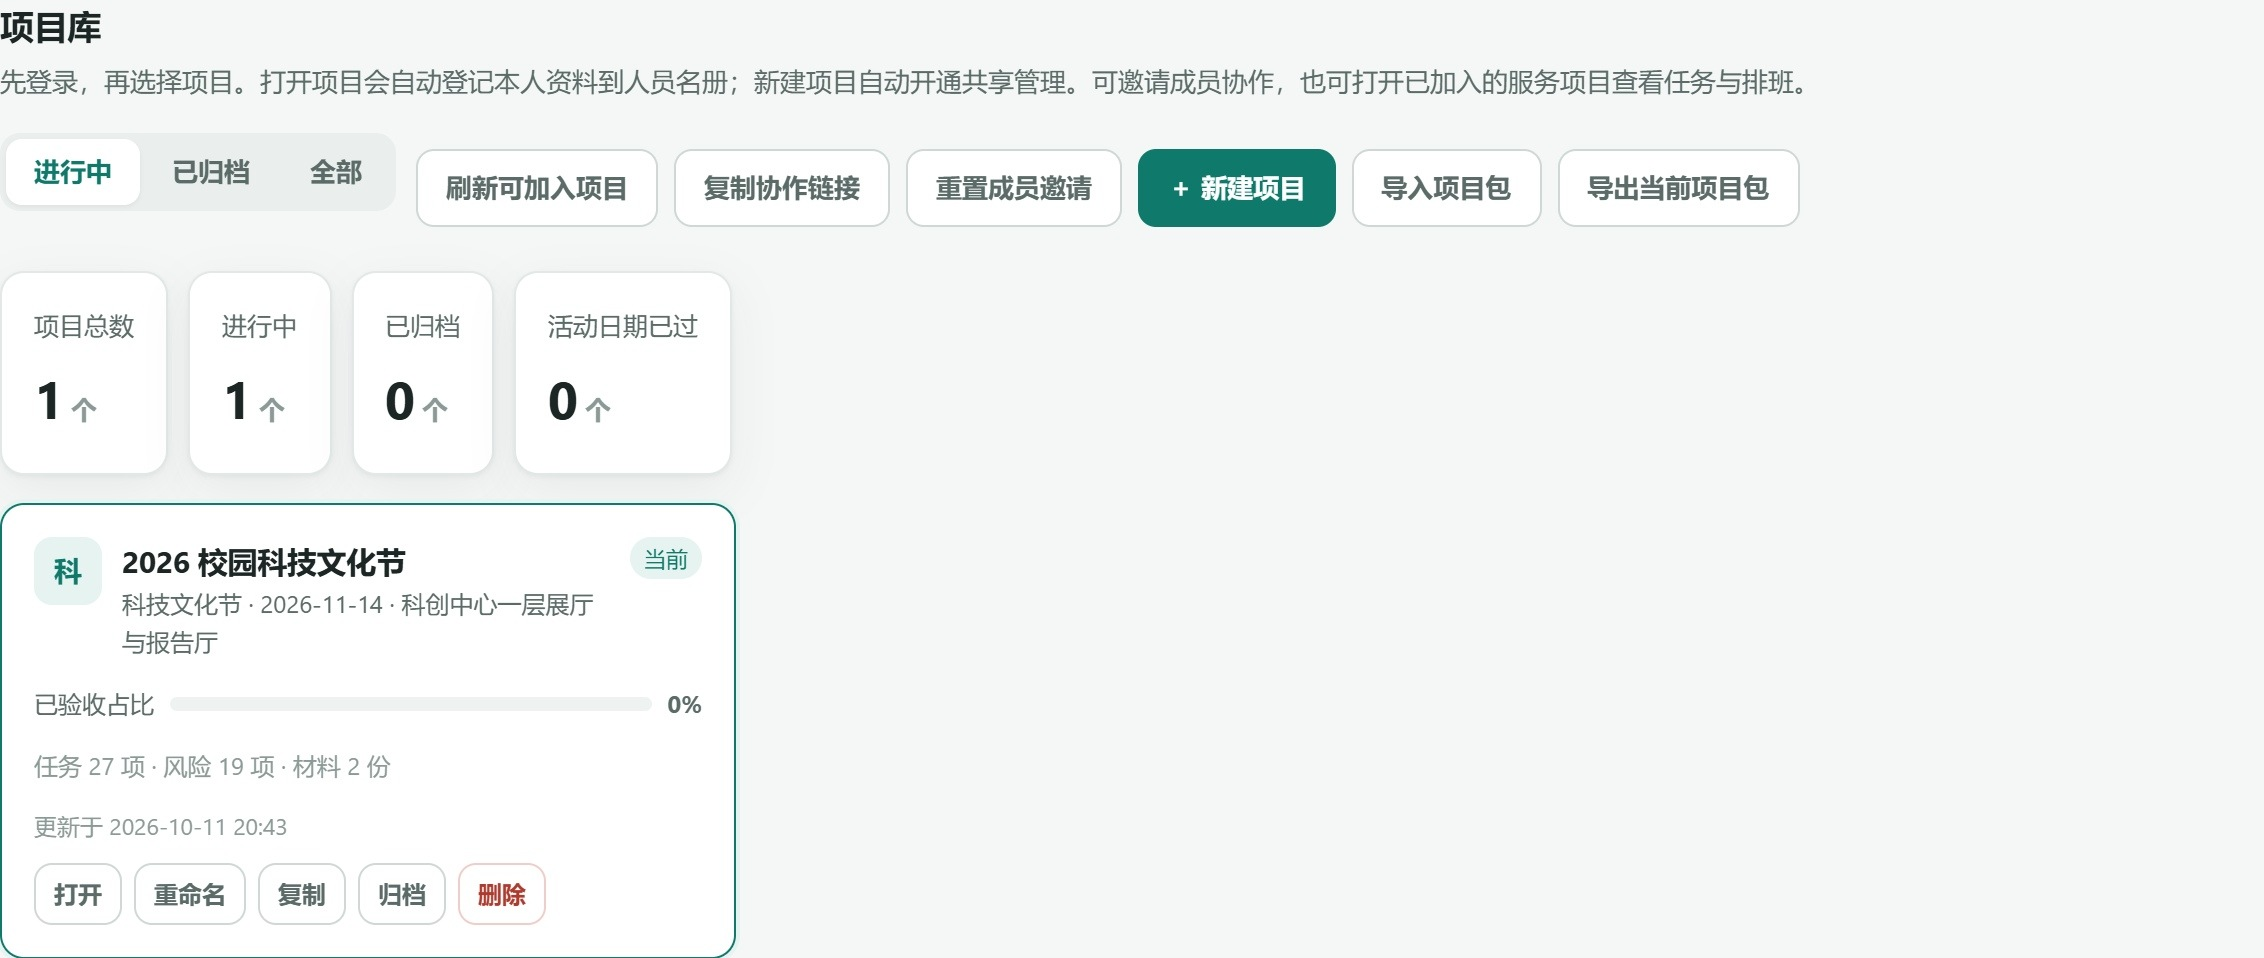
\includegraphics[width=\linewidth,height=0.28\textheight,keepaspectratio]{images/项目库.jpg}\par\vspace{3pt}{\small\color{Muted}项目库：新建、打开、邀请与导出入口}\end{center}

\Needspace{10\baselineskip}\section{活动全流程：从事实到收尾}\label{sec:2}

进入“总览”后，按填写路线图操作；顶部“引导”可跳到下一步。阶段检查点会根据现有数据提示缺口，组织者仍需核对实际准备情况。


\begingroup\small\setlength{\tabcolsep}{5pt}\renewcommand{\arraystretch}{1.28}
\begin{longtable}{>{\raggedright\arraybackslash}p{0.19\dimexpr\linewidth-6\tabcolsep\relax}>{\raggedright\arraybackslash}p{0.43\dimexpr\linewidth-6\tabcolsep\relax}>{\raggedright\arraybackslash}p{0.38\dimexpr\linewidth-6\tabcolsep\relax}}
\toprule
\textbf{阶段} & \textbf{推荐操作} & \textbf{主要结果} \\
\midrule\endfirsthead
\toprule
\textbf{阶段} & \textbf{推荐操作} & \textbf{主要结果} \\
\midrule\endhead
\bottomrule\endfoot
前期策划 & 填事实和目标；比较备选方案；分解任务并识别风险 & 策划书、方案比选、任务计划、风险台账 \\
活动筹备 & 确认人员；安排班次；核对物资；制作宣传及执行材料 & 岗位安排、物料清单、预算、宣传材料 \\
现场执行 & 查看个人任务；签到签退；记录异常；提交实际交付 & 考勤流水、班次报告、执行材料与验收记录 \\
活动收尾 & 完成任务验收；核对决算；复盘；导出并归档 & 决算表、复盘报告、项目档案 \\
\end{longtable}\endgroup

\Needspace{4\baselineskip}\subsection*{填事实与比较方案}

在“项目信息表”填写目标、对象、地点、预算、主办方、内容及约束，勾选所需产出。多日活动先选日期，再到“活动安排”为各天添加时间段和内容。问答式补全可帮助发现缺项，生成后逐条核对。


在“方案比选”中录入备选方案、评价维度、权重、分数与理由。先明确同一评分口径，再比较排名；将最终选择及理由写入策划书，避免只保留分数。


\Needspace{4\baselineskip}\subsection*{让结构化思维进入操作}

\begingroup\small\setlength{\tabcolsep}{5pt}\renewcommand{\arraystretch}{1.28}
\begin{longtable}{>{\raggedright\arraybackslash}p{0.28\dimexpr\linewidth-4\tabcolsep\relax}>{\raggedright\arraybackslash}p{0.72\dimexpr\linewidth-4\tabcolsep\relax}}
\toprule
\textbf{方法} & \textbf{在工作台中的用法} \\
\midrule\endfirsthead
\toprule
\textbf{方法} & \textbf{在工作台中的用法} \\
\midrule\endhead
\bottomrule\endfoot
SPIN、5W2H & 先厘清问题、目标与约束，再填写谁负责、何时何地、如何开展和费用 \\
MECE、WBS & 按策划、筹备、执行、收尾分组，把大目标拆成可交付任务，检查遗漏与重复 \\
ALIGN、RTGO & 为 AI 输入明确角色、目标、资料、约束和输出要求；统一不同材料的口径 \\
PDCA & 计划与排班 → 执行记录 → 交付验收 → 复盘调整，保留判断依据 \\
\end{longtable}\endgroup

\Needspace{10\baselineskip}\section{任务、人员与资源}\label{sec:3}

\Needspace{4\baselineskip}\subsection*{任务分解与责任人}

在“全周期任务”创建或生成四阶段任务，补充时间、依赖、岗位、交付物及检查点。甘特视图用于查看节奏与依赖；任务详情用于查看责任人、班次、执行记录和验收。


从已确认的项目账号名册选择实名责任人，保存后再安排执行人员。岗位文字与实名人员分开记录；填写“宣传组”等岗位名称不会自动指定某位成员。


\Needspace{4\baselineskip}\subsection*{人员加入与安排班次}

\begin{enumerate}[start=1]

\item 负责人在“人员与资源 → 服务人员”查看项目加入码，将服务入口和加入码提供给相关人员。

\item 服务人员登录，选择项目，首次输入加入码；名册显示“待确认”。负责人确认后成为“已加入”，才可正式安排。

\item 在任务行点击“安排人员”，先选任务，再勾选已确认人员。填写岗位、开始与结束时间、地点、必要技能和执行要求。

\item 需要资源时填写“每人数量”。系统按人数计算总预留，为每人生成独立班次。

\item 检查保存结果。任一人员资格、技能、时间或资源校验失败，整组不保存；修改后重新提交。

\end{enumerate}

同一人员不能在多个项目中同时排班；相邻班次可以接续。结束必须晚于开始，单班不超过 24 小时。技能由系统校验，可服务时段文字由负责人核对。已有考勤的班次应保留历史，按页面提示调整或另建安排。


\Needspace{4\baselineskip}\subsection*{资源台账与采购凭证}

在“人员与资源 → 物资与资源”登记场地、设备、物料、经费和车辆，补齐库存、已借出、计划需求、单价、地点、来源和状态。净可用量为库存减已借出；维修或报废资源不能预留。重叠班次按同时使用的峰值检查，前后使用无需简单累加。


“计划需求”表示活动总体需求，班次预留表示具体时段安排，两者不要相加。修改库存后，负责人应重新核对已排班次。


“过程材料”中的物料清单由资源台账生成，提供只读查看和 Word、Excel、Markdown 导出。需要改数量时回到资源台账，避免两套清单不一致。


采购凭证可在资源行上传或拖入文件，每项最多 6 份。400 KB 以内原件随项目包保存，可下载；超过上限时仅记录文件名，原件另存。Excel 导出列出凭证文件名，原件从台账下载。预算与决算表也保留逐行发票入口。


\Needspace{10\baselineskip}\section{材料制作与 AI 工作流}\label{sec:4}

\Needspace{4\baselineskip}\subsection*{生成、编辑与确认版本}

\begin{enumerate}[start=1]

\item 在“项目信息表”勾选产出；进入“过程材料”打开对应卡片。系统提供策划书、宣传文案、执行手册、预算、复盘等 21 类内置产出，并可自定义。

\item 文本生成使用 DeepSeek。先检查引用的活动事实、任务、风险及资料，再生成正文；也可以直接手工撰写。

\item 在“在线编辑”修改段落和表格，或切换“Markdown 源码”。金额表的合计与占比按内容计算，派生单元格不能直接修改。

\item 核对名称、日期、数字、责任人和事实来源；点击“确认并保存交付版本”，保存可用于任务提交的版本。

\item 选择 Word、Excel 或 Markdown 导出。文件导出用于交付，项目 JSON 用于保存整体项目。

\end{enumerate}

\begin{center}
\includegraphics[width=\linewidth,height=0.28\textheight,keepaspectratio]{images/材料版本.jpg}\par\vspace{3pt}{\small\color{Muted}过程材料：草稿编辑、版本确认与文档导出}\end{center}

\textbf{AI 生成结果与人工编辑正文仍是草稿。} 确认版本保存当时的正文及已存附件等快照；后续编辑、改名或再次生成不会替换历史交付版本。


\Needspace{4\baselineskip}\subsection*{使用参考表与生成宣传图}

上传 \path{.docx} 参考件后，可按栏目填写或使用“参考表填值”。挂有原表时，“Word（参考原表）”导出填好的原表，“Word（正文）”导出正文版本。复杂模板先试导出并检查布局。


海报使用 GPT-image2。先准备活动事实、宣传文案、视觉要求和附加约束，核对装配后的提示词，再点击生图。完成后检查文字、日期和画面内容，下载原图并在素材库登记。没有配置 AI 时，手工编辑、项目管理与导出仍可使用。


\Needspace{4\baselineskip}\subsection*{知识库、素材库与卡片工作流}

在“知识与素材”中切换知识库或素材库，导入文本、Word 或登记图片、链接。填写来源、适用阶段和内容说明；审核后勾选“用于 AI 生成”。图片补充视觉描述，链接补充核实后的摘要，帮助 AI 准确引用。资料内容修改后重新审核和选择。


在“卡片工作流”中新建卡片，选择技能、输入资料、上游卡片和额外要求。例如先整理统一口径，再分别生成通知与岗位简报。运行全部时按依赖执行；上游失败时先处理失败卡片，再运行下游。


检查结果后点击“写入过程材料”。覆盖已有正文前确认保留旧稿；写入后仍需编辑核对并确认交付版本。生成不是验收，工作流也不会自动完成任务。


\Needspace{10\baselineskip}\section{现场执行、风险与交付验收}\label{sec:5}

\Needspace{4\baselineskip}\subsection*{服务人员的个人操作}

服务人员进入“我的任务”，查看本人岗位、关联任务、时间、地点、要求与资源，依次接受班次、到岗签到、离场签退，并填写班次执行报告。负责人可按授权代打卡，系统记录操作者。


工时按服务器记录的有效“签到 → 签退”时段累加；未签退的在场时间单独显示。服务人员班次与普通参与者表单分别管理。


\Needspace{4\baselineskip}\subsection*{整项任务如何完成}

任务按“未开始 → 进行中 → 待验收 → 已验收”推进，受阻原因独立记录。


\begin{enumerate}[start=1]

\item 责任人检查安排与条件，点击“开始执行”。

\item 完成工作并整理材料，在“过程材料”确认实际交付版本。

\item 在任务详情点击“提交验收”，选择真实材料版本并填写交付说明。

\item 组织者核对提交版本，写明结论，验收通过或退回补充。

\item 被退回后修改材料、确认新版本，再次提交。既有验收仍绑定原提交版本，不会被新稿替换。

\end{enumerate}

\begin{center}
\includegraphics[width=\linewidth,height=0.28\textheight,keepaspectratio]{images/任务验收.jpg}\par\vspace{3pt}{\small\color{Muted}任务详情：责任人、班次记录与提交验收入口}\end{center}

\textbf{班次报告、签到时长和整项任务验收分别记录。} 确认交付、提交和验收需要登录已确认的项目账号；旧任务提示“待补充”或“待核实”时，先补人员与版本依据，再完成验收。


\Needspace{4\baselineskip}\subsection*{全流程风险与变更演练}

在“风险预案”中添加或生成风险，逐项填写阶段、类别、关联任务、责任角色、触发信号、预防、响应及升级路径。可能性和影响各按 1 至 5 分评定，风险分值为两者乘积：低风险 1 至 7 分，中风险 8 至 14 分，高风险 15 至 25 分。


点击风险矩阵筛选重点，查看覆盖度自检提示；按实际依据评估，避免为了满足分布提示而调整真实风险。导出分级应急预案与应急处置卡，核对现场联络人与升级链。到“变更演练”选择场景，逐步记录决策、行动和结论，必要时写回风险台账并调整任务。


\Needspace{4\baselineskip}\subsection*{参与者报名与签到}

在“参与者”配置字段、必填和去重规则，开启收集。确认访问地址后生成链接或二维码，让参与者填写；在工作台查看汇总、修正记录、签到及导出 CSV、JSON。


手机访问必须使用可达的局域网地址或 HTTPS 地址，不能把 \path{127.0.0.1} 发给手机。地址变化后重新生成二维码。提交页面显示“本机已保存”或“正在发送”时尚未确认送达；以“已直达组织者电脑”为准，未送达可按页面重试或用回执码、CSV 补录。结束收集后关闭表单。


\Needspace{10\baselineskip}\section{多人协作与收尾归档}\label{sec:6}

\Needspace{4\baselineskip}\subsection*{成员协作}

组织者在“项目库”复制协作链接，按需提供编辑或只读邀请。成员登录各自账号后打开链接，查看顶部共享角色、版本和同步状态。课堂模拟可用不同浏览器或隐私窗口，避免多个标签共用同一账号状态。


同组先约定分工，尽量在不同任务或材料上编辑。出现版本冲突时：先下载本地草稿，再加载共享最新版本，人工合并差异，核对后保存。不要直接覆盖未备份的本地修改。组织者重置邀请后，旧链接失效。


把项目切换为本地副本后，原共享项目仍单独存在。换设备前保留组织者凭据；组织者管理入口使用原管理凭据。局域网和跨网络开通方法见《运维指南》第 3 节。


\Needspace{4\baselineskip}\subsection*{活动结束后的归档}

\begin{enumerate}[start=1]

\item 核对所有班次签退、任务验收、资源归还、凭证和决算。

\item 在收尾材料中记录目标达成情况、问题、处置及复盘结论。

\item 导出所需 Word、Excel、Markdown 等成果文件。

\item 导出完整项目 JSON；在服务人员区导出人员、班次与考勤 JSON，在参与者区导出报名记录。

\item 单独保存海报原图、大附件、参考原件。完成服务器备份后，在项目库归档。

\end{enumerate}

项目包导入可恢复其中保存的项目内容；账号、密码、服务器班次和考勤须通过完整服务端备份恢复。人员档案 JSON 用于复核归档，账号恢复按运维指南操作。


\Needspace{10\baselineskip}\section{常见问题速查}\label{sec:7}

\begingroup\small\setlength{\tabcolsep}{5pt}\renewcommand{\arraystretch}{1.28}
\begin{longtable}{>{\raggedright\arraybackslash}p{0.28\dimexpr\linewidth-4\tabcolsep\relax}>{\raggedright\arraybackslash}p{0.72\dimexpr\linewidth-4\tabcolsep\relax}}
\toprule
\textbf{现象} & \textbf{处理方法} \\
\midrule\endfirsthead
\toprule
\textbf{现象} & \textbf{处理方法} \\
\midrule\endhead
\bottomrule\endfoot
注册提示“API 路径不存在” & 可能连接旧后端；运行 \path{start.bat} 后刷新，仍失败交维护者检查 \\
AI 按钮不可用 & 联系维护者检查对应服务配置；可先手工编辑和导出 \\
服务人员无法安排 & 先确认入组，再查技能、时间冲突及资源库存；失败批次不会部分保存 \\
做完班次后任务仍未完成 & 进入任务详情，选择已确认交付版本提交，再由组织者验收 \\
成员不能编辑 & 检查邀请角色、顶部同步状态及账号资格；只读链接需由组织者更换 \\
手机扫码打不开或未送达 & 检查地址和网络；重发二维码，查看实际送达提示，必要时补录 \\
换浏览器后本地项目不见了 & 本地项目与浏览器关联；使用原浏览器导出的项目包，或有效共享邀请 \\
忘记密码 & 核对账号与输入，联系维护者协助处理 \\
\end{longtable}\endgroup

操作中遇到未列出的报错，保留报错文字、所在页面和操作步骤，先导出项目，再联系维护者。

\end{document}
